\documentclass[14pt, a4paper]{book}
\begin{document}

Now is the time to focus on the critical task of preparing the data for our DM search using ML. This task is essential because accurately distinguishing between signal and background events is a key challenge in searching for any new signal event, 
as seen on Section \ref{sec:data_anal}. In this chapter we will define what \textit{background} and \textit{signal} actually are, as well as selecting appropriate kinematical cuts to define the control region for our search. In addition we will 
explain the data preparing procedure such that it is in a format that is well-suited for our ML algorithms. The reason this process is of great importance is because we can maximize the chances of our ML agrorithm to accurately identify any DM signals. 
Moreover, by providing a detailed explanation of the data preparation process, we can ensure that our dataset is both reliable and effective, and that our analysis is robust and trustworthy. In short, this chapter represents a critical step towards 
achieving our goal of using ML to classify DM from SM events using ATLAS data, and it is essential to the success of our overall research goal.



\clearpage
\section{Standard Model background estimation}
As we are going to look at dilepton final states with missing trasnverse energy to try to teach our ML to learn DM signatures, then we need to take into account all possible SM background event that have these kind of final states. The SM backgrounds processes we will look at are explained in the next subsections.

\subsection{W and Drell Yan}
$W/Z/\gamma^*$+jets as all of these can directly decay into two leptons, $W/Z/\gamma\rightarrow ll'$, where the prime marks a different flavour. All the production mechanism for these background processes can 
be seen in Figure \ref{fig:WZG_BKG}. As the $W$ boson behaves differenty than the $Z$ and $\gamma$, since the $W$ boson can decay into neutrinos giving us MET, while the $Z$ and $\gamma$ processes have the highest cross section. We will divide 
these background processes into two, $W$ and $Z/\gamma^*$ + jets, also called \textit{Drell Yan} processes. To simulate these background processes Sherpa 2.2.11 \cite{Sherpa} was used.
\graphicspath{{../../figures/}}
\begin{figure}[!ht]
    \centering
    \includegraphics[width=\textwidth]{WZGjetsBKG.png}
    \caption[$W/Z/\gamma$+jets production]{Diagrams showcasing SM $W/Z/\gamma$+jets production. A quark marked with a prime, indicated that the quark might be a diferent flavour after interacting with a boson.}\label{fig:WZG_BKG}
\end{figure}

\subsection{TTbar}
Another SM background process we will look at are processess that have a $t\bar{t}$ in them. Since the top has a high branching ratio of decaying into a $b$-quark and a $W$ boson, $t\rightarrow bW^+$, where the $W$ boson can again decay into a neutrino giving 
us MET. The main production mechanism for these processes can be seen in Figure \ref{fig:TT_BKG}. To simulate these background processes Powheg-Box v2 \cite{PowHeg} interfaced with Pythia 8 \cite{Pythia} was used.
\begin{figure}[!ht]
    \centering
    \begin{subfigure}[b]{0.3\textwidth}
        \centering
        \includegraphics[width=\textwidth]{TTBar1.png}
        \caption{$s$-channel}
    \end{subfigure}
    \hfill
    \begin{subfigure}[b]{0.3\textwidth}
        \centering
        \includegraphics[width=0.9\textwidth]{TTBar2.png}
        \caption{Gluon fusion}
    \end{subfigure}
    \hfill
    \begin{subfigure}[b]{0.3\textwidth}
        \centering
        \includegraphics[width=\textwidth]{TTBar3.png}
        \caption{$t$-channel}
    \end{subfigure}
    \caption[$t\bar{t}$ production]{Diagrams showcasing SM $t\bar{t}$ production}\label{fig:TT_BKG}
\end{figure}

\subsection{Single top}
On the same note we have processes with a single top. Where again the the top has a high branching ratio of decaying into a $b$-quark and a $W$ boson, $t\rightarrow bW^+$, where the $W$ boson can again decay into a neutrino giving 
us MET. The main production mechanism for these processes can be seen in Figure \ref{fig:T_BKG}. To simulate these background processes Powheg-Box v2 \cite{PowHeg} interfaced with Pythia 8 \cite{Pythia} was used.
\begin{figure}[!ht]
    \centering
    \begin{subfigure}[b]{0.3\textwidth}
        \centering
        \includegraphics[width=\textwidth]{SingleTop1.png}
        \caption{$s$-channel}
    \end{subfigure}
    \hfill
    \begin{subfigure}[b]{0.3\textwidth}
        \centering
        \includegraphics[width=\textwidth]{SingleTop2.png}
        \caption{$t$-channel}
    \end{subfigure}
    \hfill
    \begin{subfigure}[b]{0.3\textwidth}
        \centering
        \includegraphics[width=\textwidth]{SingleTop3.png}
        \caption{$tW$}
    \end{subfigure}
    \caption[Single Top production]{Diagrams showcasing SM single top productions.  A quark marked with a prime, indicated that the quark might be a diferent flavour after interacting with a boson.}\label{fig:T_BKG}
\end{figure}

\newpage\subsection{Diboson}
The last SM bacgkround process we will look at are processes containing two bosons, called \textit{diboson} backgrounds. The two SM bosons we will consider when looking into these final states are the $W$ and $Z$, as these can decay as $W/Z\rightarrow ll'/ll$ 
or $W\rightarrow l\nu_l$, where the prime means a different lepton flavour. The main production mechanism for these processes can be seen in Figure \ref{fig:Diboson_BKG}. To simulate these background processes Sherpa 2.2.11 \cite{Sherpa} was used.
\begin{figure}[!ht]
    \centering 
    \begin{subfigure}[b]{0.4\textwidth}
        \centering
        \includegraphics[width=\textwidth]{Diboson1.png}
        \caption{$s$-channel $WZ$}
    \end{subfigure}
    \hfill
    \begin{subfigure}[b]{0.4\textwidth}
        \centering
        \includegraphics[width=\textwidth]{Diboson2.png}
        \caption{$s$-channel $WW$}
    \end{subfigure}
    \hfill
    \begin{subfigure}[b]{0.4\textwidth}
        \centering
        \includegraphics[width=\textwidth]{Diboson3.png}
        \caption{$t$-channel $WZ$}
    \end{subfigure}
    \hfill
    \begin{subfigure}[b]{0.4\textwidth}
        \centering
        \includegraphics[width=\textwidth]{Diboson4.png}
        \caption{$t$-channel $WW$ and $ZZ$}
    \end{subfigure}
    \caption[Diboson production]{Diagrams showcasing SM diboson production. A star superspcript on a boson indicates that the boson needs to be virtual and off mass shell.  A quark marked with a prime, indicated that the quark might be a diferent flavour after interacting with a boson. }\label{fig:Diboson_BKG}
\end{figure}

\section{Dark Matter samples}

\section{Object selection}\label{sec:obj_sel}
Before getting into our DM search and regions we will study we have to define how standard objects are defined. By standard objects it is meant leptons, jets, etc. As this thesis is made using ATLAS data and simulations we will use the same standard crietria 
cuts they choose.\\
\\The electrons are selected using the criteria on Table \ref{tab:E_selec}.
\begin{table}[!h]
    \centering\caption[Electron selection criteria]{Electron selection criteria.}
    \begin{tabular}{l|r}\midrule\midrule
        Feature                                                                 & Selection criteria        \\\midrule
        Transverse momentum                                                     & $p_T > 25$ GeV     \\
        Pseudorapidity range                                                    & $\abs{\eta}<1.37$ or  $1.52<\abs{\eta}<2.47$ \\
        $d_0$ significance cut                                                  & $\abs{d_0^{BL}(\sigma)}<5$    \\
        $z_0$ cut                                                               & $\abs{\Delta z_0^{BL}\sin\theta}<0.5$mm    \\\midrule\midrule
    \end{tabular}
    \label{tab:E_selec}
\end{table}
\\The muons are selected using the criteria on Table \ref{tab:mu_selec}.
\begin{table}[!h]
    \centering\caption[Muon selection criteria]{Muon selection criteria.}
    \begin{tabular}{l|r}\midrule\midrule
        Feature                                                                 & Selection criteria        \\\midrule
        Transverse momenum                                                      & $p_T > 27(20)$ GeV for leading (subleading)     \\
        Pseudorapidity cut                                                      & $\abs{\eta}<2.5$ \\
        $d_0$ significance cut                                                  & $\abs{d_0^{BL}(\sigma)}<5$    \\
        $z_0$ cut                                                               & $\abs{\Delta z_0^{BL}\sin\theta}<0.5$mm    \\\midrule\midrule
    \end{tabular}
    \label{tab:mu_selec}
\end{table}
\\The jets are selected using the criteria on Table \ref{tab:jet_selec}.
\begin{table}[!h]
    \centering\caption[Jet selection criteria]{Jet selection criteria.}
    \begin{tabular}{l|r}\midrule\midrule
        Feature                                                                 & Selection criteria        \\\midrule
        Algorithm                                                               & Anti-$k_t$     \\
        $R$-parameter                                                           & 0.4     \\\midrule
        Transverse momentum                                                     & $p_T > 20$ GeV     \\
        Pseudorapidity cut                                                      & $\abs{\eta}<4.5$ \\
        Jet Vertex Tagger                                                       & $>0.5$ for $p_T<60$ GeV, $\abs{\eta}<2.4$ \\
        forward JVT                                                             & fJVT $<0.4$ and |timing| < 10 ns for $p_T<120$ GeV, $2.5<\abs{\eta}<4.5$ \\\midrule
        b-jet tagging                                                           & DL1r score > 0.665 with 85\% efficiency \\\midrule\midrule
    \end{tabular}
    \label{tab:jet_selec}
\end{table}
% \\The missing transverse energy is reconstructed from jets selected and calibrated according to the information in Table \ref{tab:jet_selec}



\section{Control region}
Now that we have defined what our background and signal are, the next step is to create a so-called \textit{control region}. The control region is the kinematical region we will use as a base for our search. As we are conducting a model inedpendent search we want 
our kinematical cuts to be minimal and as general as possible. As we are looking at a dilepton final state, then we need to first define what we mean by that. If we were only searching for DM with the $Z'$ model, then a sensible definition would be a 
Same Flavour Opposite Sign (SFOS) leptons ($e^\pm e^\mp, \mu^\pm\mu^\mp$). However to stay as general, and model independet, as possible we will also study other possible combinations as these might be important for theories such as SUSY or Lepton Flavour Violating 
(LFV) models. These are Different Flavour Same Sign (DFSS), DFOS and SFSS lepton pairs.\\
\\Since we are looking for DM, which we expect to behave similarly to a neutrino, then a nice kinematical variable to set a general cut to isolate signal from background is the MET, we can see the 
distribution of MET on all of Run II in a dilepton final state in Figure \ref{fig:uncut_met}.
\graphicspath{{../../../Plots/Data_Analysis/SRs/Uncut/}} 
\begin{figure}[!ht]
    \centering
    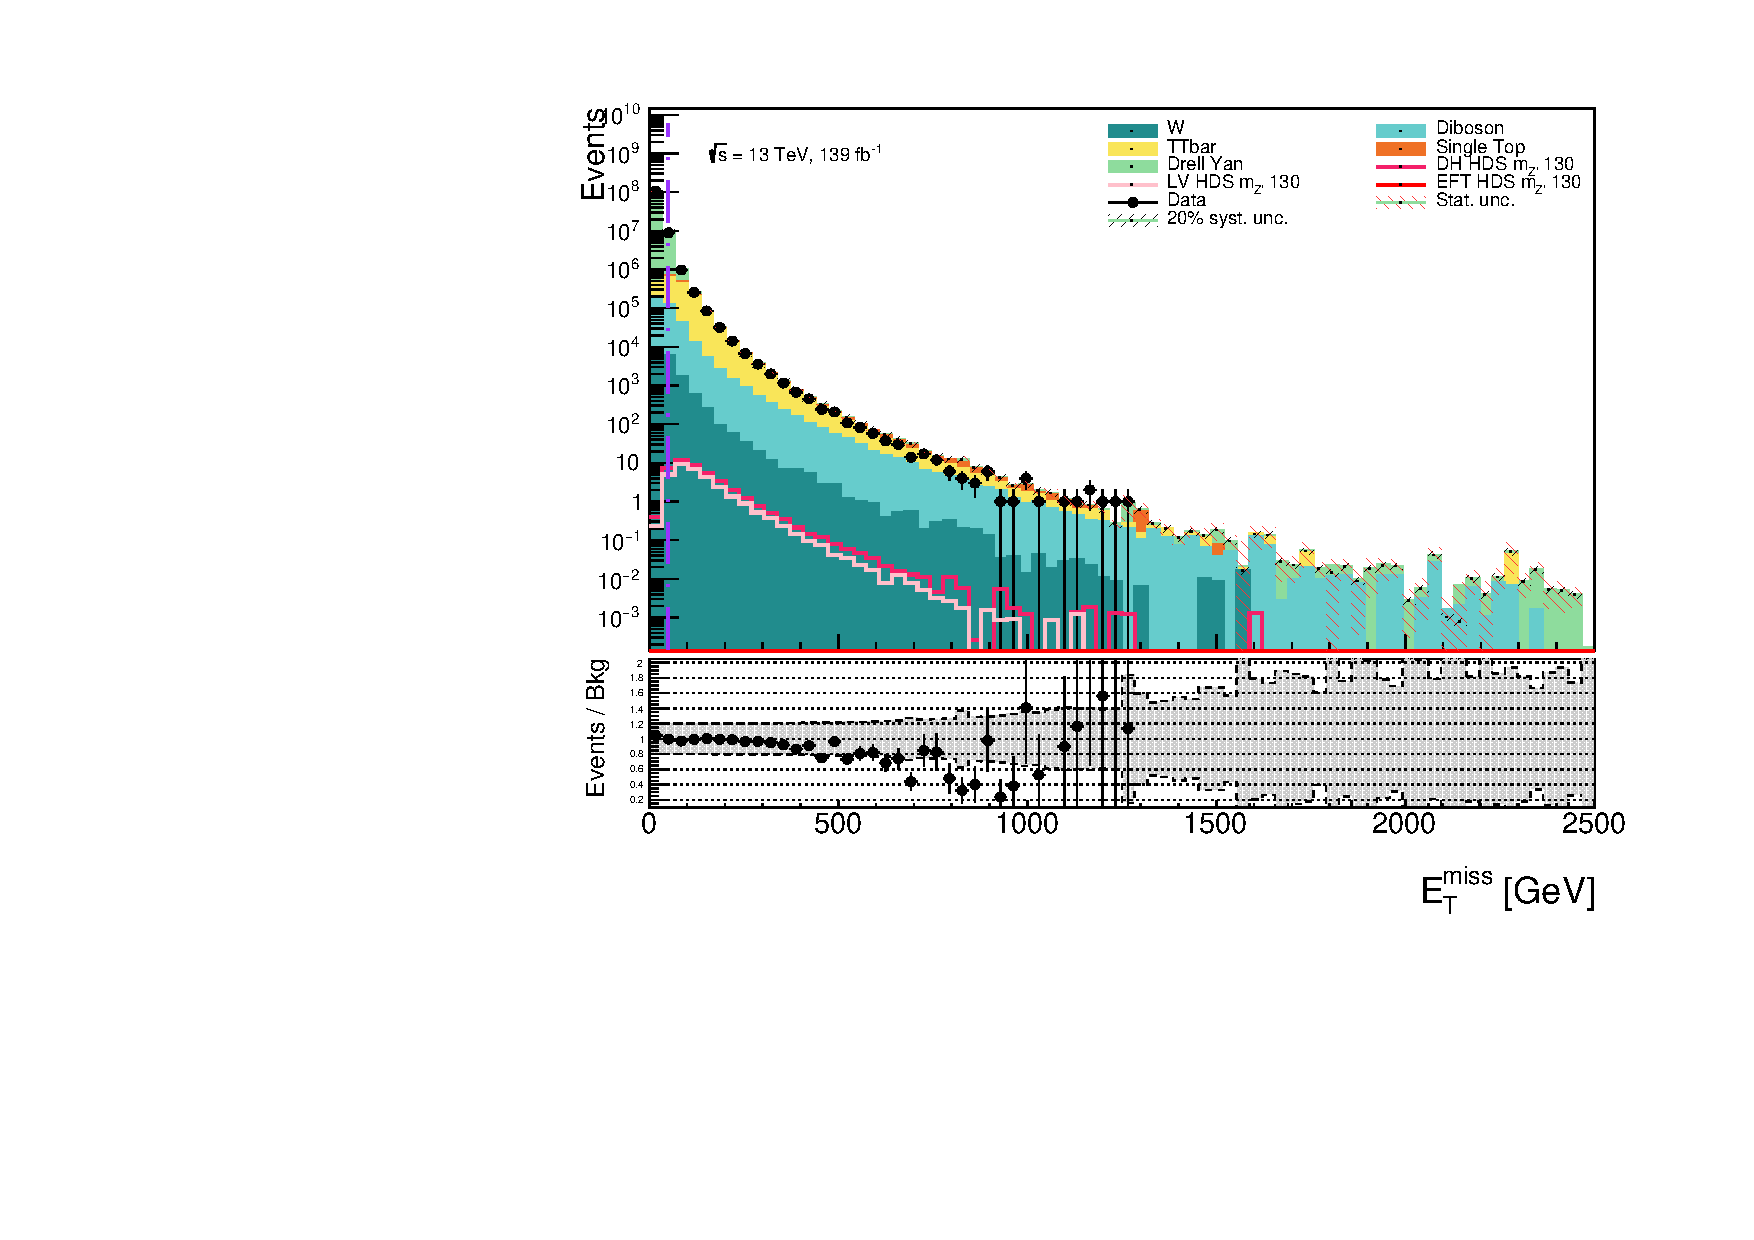
\includegraphics[width=1\textwidth]{met.pdf}
    \caption[MET dilepton final state Run II]{Distribution of MET when looking at a dilepton final state in all of Run II}\label{fig:uncut_met}
\end{figure}
\\As we are conducting a model independent search, we want to use minimal cuts. The MET cut made in this thesis was chosen to be of 50 GeV, meaning we will \textit{only} look at events where the MET is greater than this. 
This both because of the amount of events that are in a dilepton final state, and also because most models studied in this thesis have roughly more MET than 50 GeV.\\
\\Another kinematical cut that will be included in this thesis is another jet $p_T$ on top of the one from Table \ref{tab:jet_selec}. This is because jet reconstruction is already a hard task, but when pushing the limits of our selection criteria with a MET cut 
becomes even harder. And the worse the reconstruction of the jets the worse the agreement between MC simulations and real data is, and as we already know, the SM agrees with what we observe with an incredible accuracy. In Figure \todo{MAKE THE IMAGE} we can see 
how the data and MC simulations of the SM agree when ounting the number of jets with different $p_T$ cuts. \\
\\Other than the object selection criteria, these are the only cuts that will be used to define the control region. Their summary can be seen in Table \ref{tab:CR_cuts}
\begin{table}[!h]
    \centering\caption[Control Region for model-indepentent search]{Table showcasing the cuts used to define our model independent search.}
    \begin{tabular}{l|r}\midrule\midrule
        Feature                                                                 & Selection criteria        \\\midrule
        Dilepton final state                                                    & $\ell^\pm \ell^\mp$, $\ell^\pm \ell^\pm$, $\ell^\pm \ell'^\mp$ and $\ell^\pm \ell'^\pm$    \\
        Missing Transverse Energy                                               & $E_T^{miss} > 50$ GeV     \\
        Light jets                                                              & $p_T > 40$ GeV     \\\midrule\midrule
    \end{tabular}
    \label{tab:CR_cuts}
\end{table}


\clearpage
\section{Feature selection for ML}
For this thesis there are many possible kinematic variables that can be used as features for our ML algorithms, in this section we will make use of the kinematical variables presented in Section \ref{sec:particle_kinematics} as well as introduce new variables that 
might help our ML algorithm to correctly learn the patters of SM bacgkround and DM signal events. \\
\\As we are stuyding a final state with two leptons it is therefore natural to look at the kinematics for both of these as these will give us as general information as possible. The first thing we will look at is the transverse momentum, $p_T$, of each lepton as defined in Eq. (\ref{eq:transverse_momentum}). 
We will also look at the azimuthal angle, $\phi$ and the pseudorapidity, $\eta$ defined in Eq. (\ref{eq:pseudorapidity}), to know where in the detector the leptons are located. 
With this we have practically constructed a four-momentumv from which we could learn all particle kinematics. However, we want to help our ML algorithm as much as possible in the task of learning SM background and DM signal. A powerful kinematical varable for this is 
therefor the invariant mass, $m_{ll}$ defined in Eq. (\ref{eq:invariant_mass}), which can help the ML algorithm sort out resonant models. Another variable of interest is the trnsverse energy, $E_T$ defined in Eq. (\ref{eq:transverse_energy}) for the lepton pair. 
The distribution of the invariant mass can be seen in Figure \ref{fig:mll_dist}.
\graphicspath{{../../../Plots/Data_Analysis/SRs/Control_region/}} 
\begin{figure}[!ht]
    \centering
        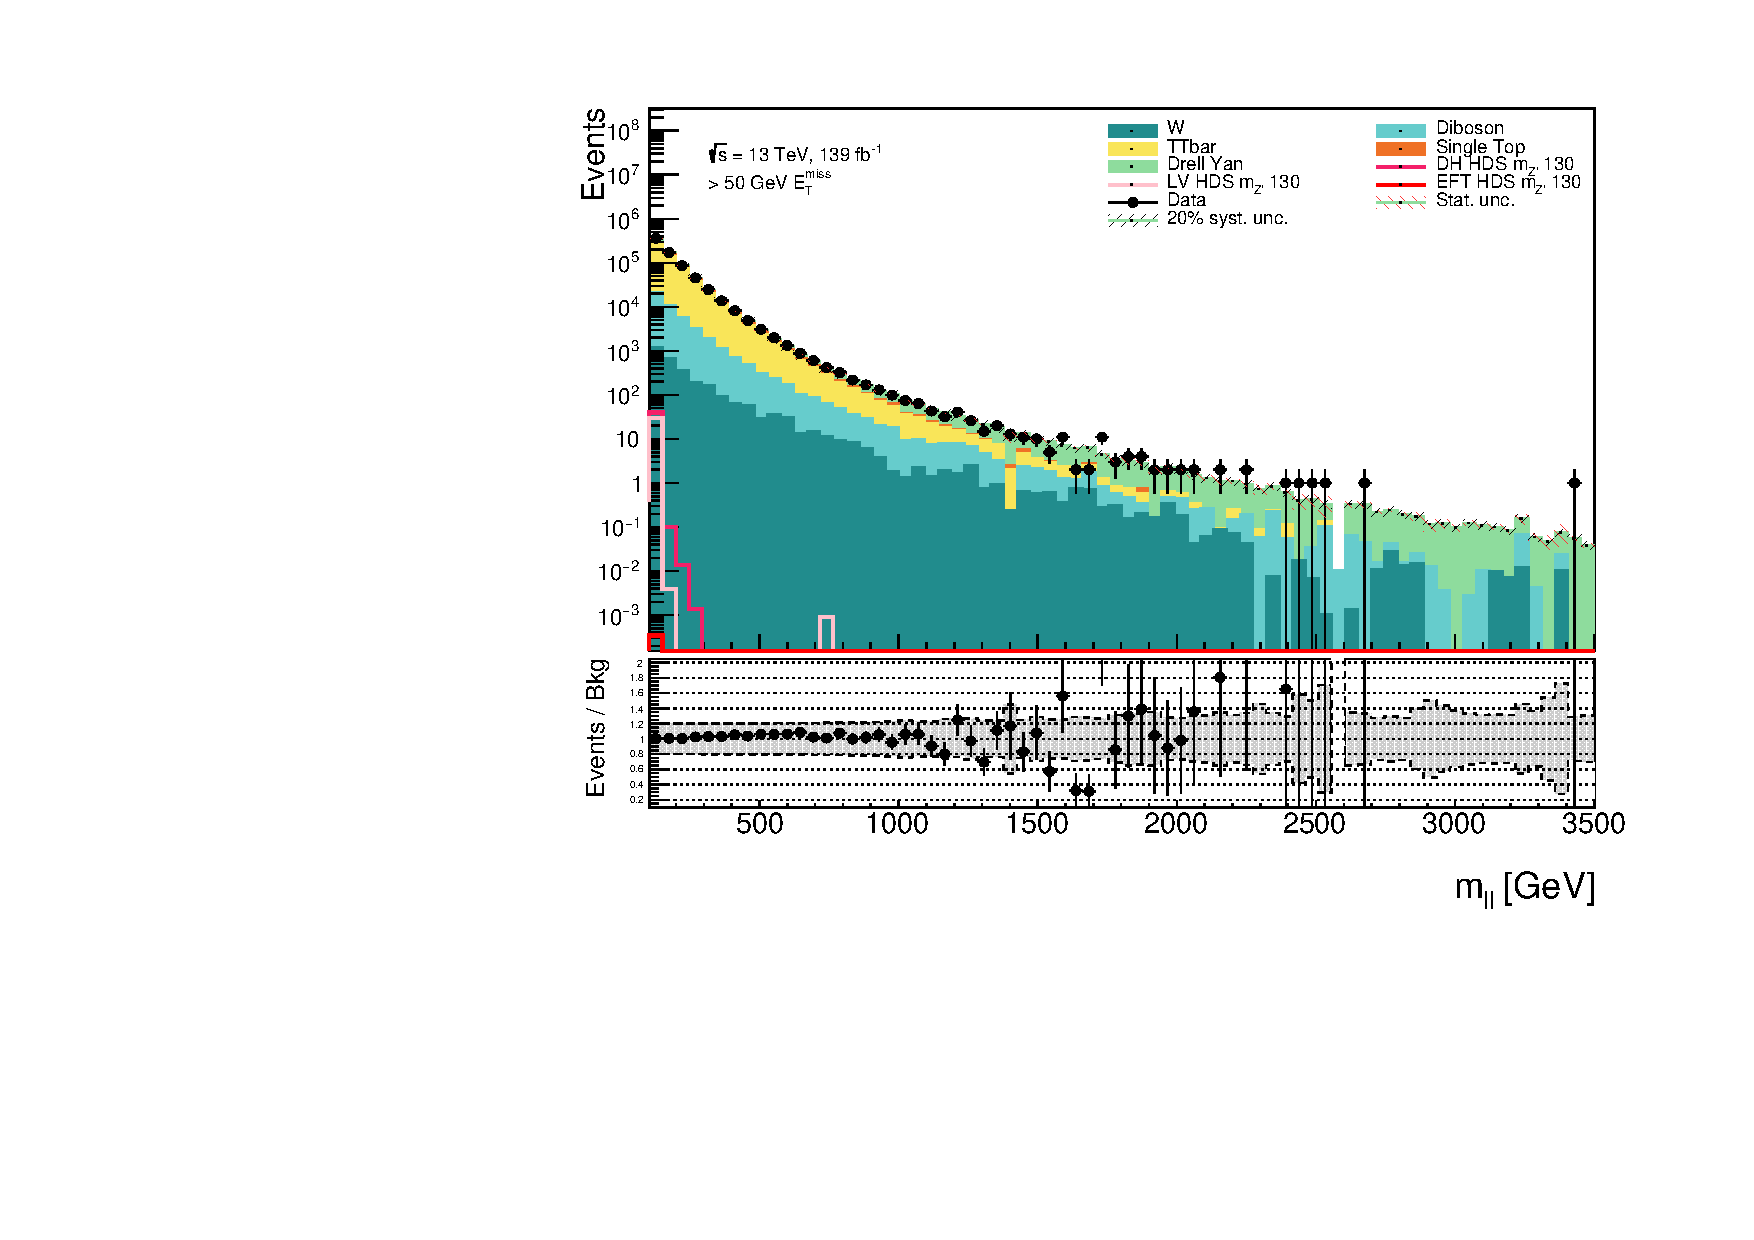
\includegraphics[width=0.8\textwidth]{mll.pdf}
    \caption{Distribution of $m_{ll}$ in control region.}\label{fig:mll_dist}
\end{figure}
\\As we are studying DM, an invisible particle, the most important kinematical variable to distinguish background from signal is the missing transverse energy, $E_T^{miss}$ defined in Eq. (\ref{eq:MET}), as this how we expect DM to be recorded.
Another version of the MET is the so-called \textit{Object-based $E_T^{miss}$ significance}, or $E_T^{miss,sig}$ for short, this variable is used tto deal with artifical or fake $E_T^{miss}$. The way $E_T^{miss,sig}$ works is by 
weighing the the value of $E_T^{miss}$ by the precision of its reconstruction. It is defined as
\begin{equation}\label{eq:METsig}
    E_T^{miss,sig} = \frac{E_T^{miss}}{\sigma(E_T^{miss})}
\end{equation}
where $\sigma(E_T^{miss})$ is the uncertainty of the reconstruction of the $E_T^{miss}$, which consider the indidual uncerainties of the objects that enter the $E_T^{miss}$ calcuation. The distribution of this variable can ve seen in Figure \ref{fig:met_sig_dist}. 
In this thesis we will use both $E_T^{miss}$ and $E_T^{miss,sig}$ even though they are correlated, as the algorithm might chose in different instances\footnote{Meaning different \textit{signal reagions} when conducting a model independent search. See Chapter TO COME} 
which of these is of more importance.
\begin{figure}[!ht]
    \centering
        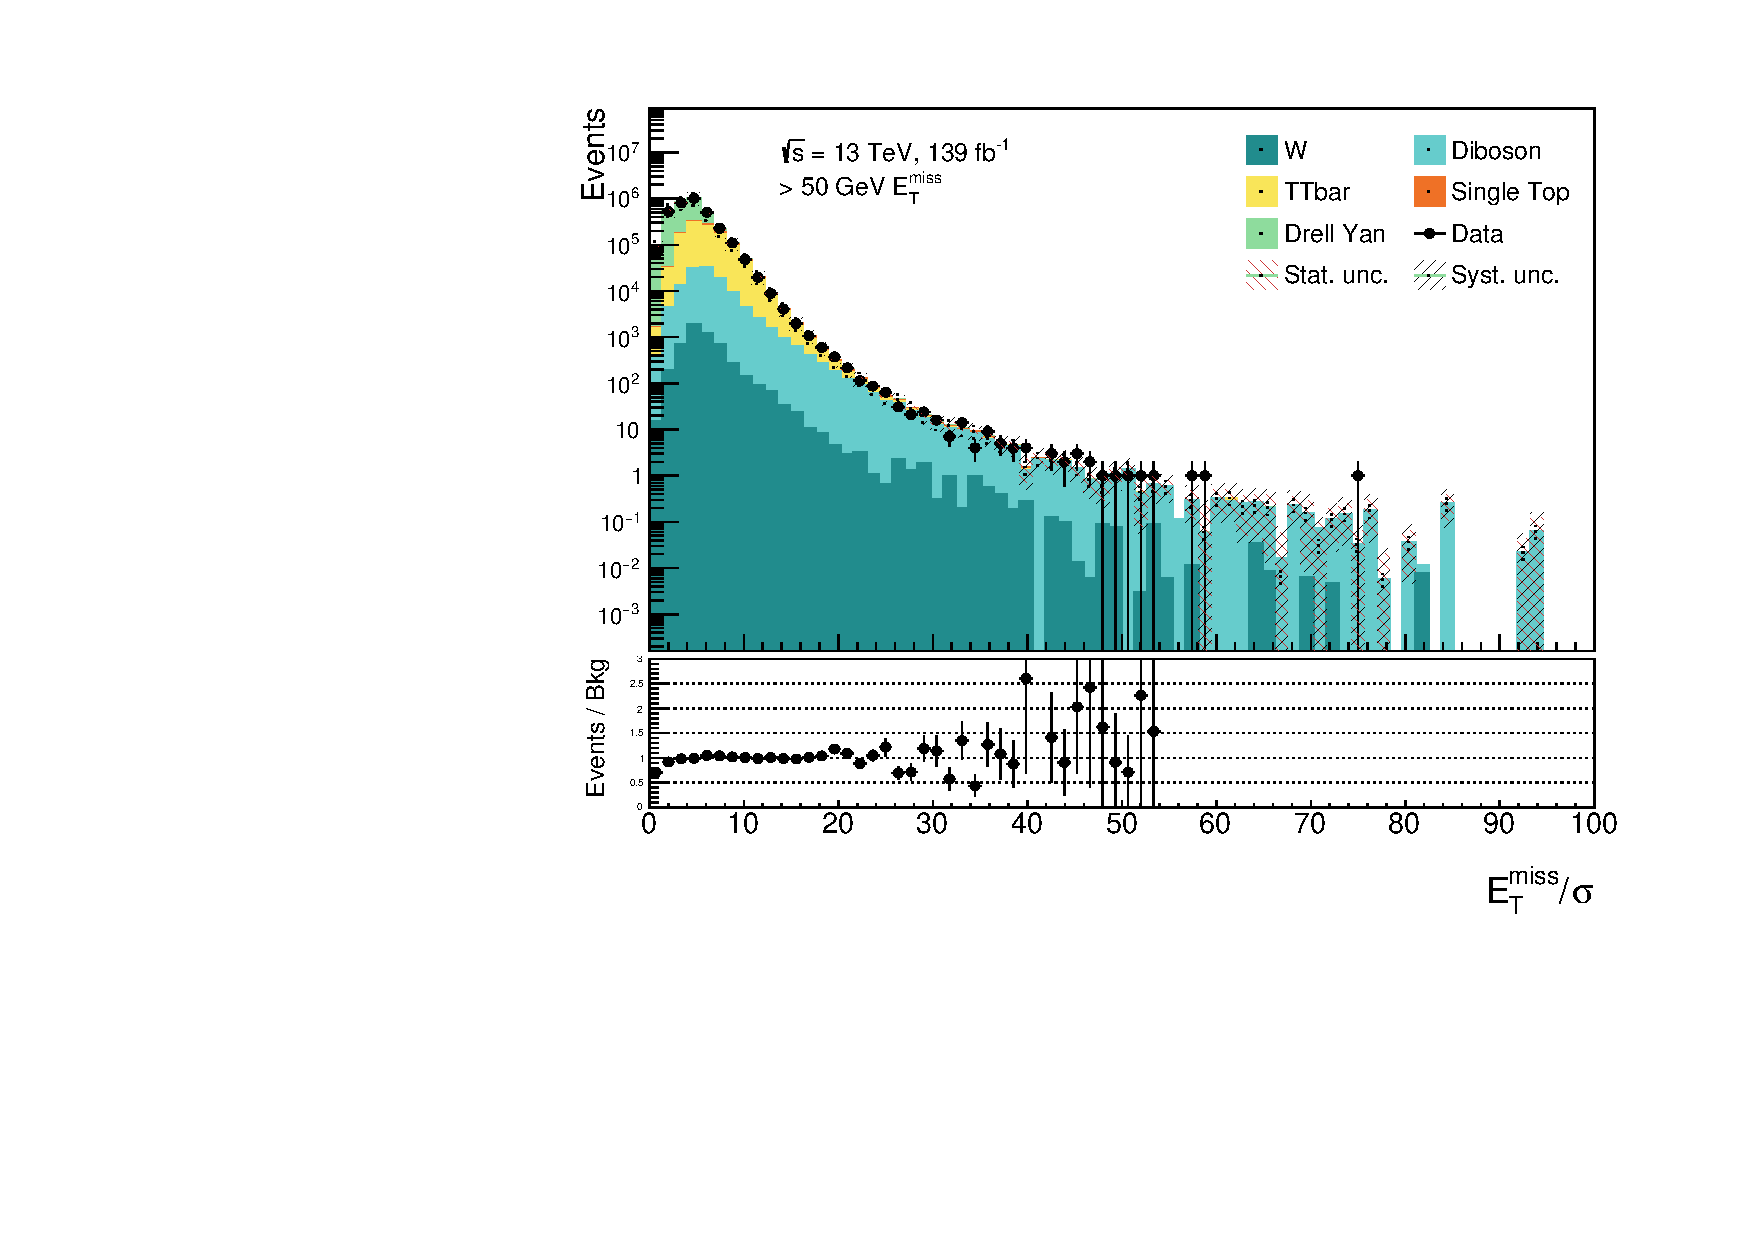
\includegraphics[width=0.8\textwidth]{met_sig.pdf}
    \caption{Distribution of $E_{T}^{miss,sig}$ in control region.}\label{fig:met_sig_dist}
\end{figure}
\\To keep the trend of variables for invisible particles, we will also study the transverse mass, $m_T$ defined in Eq. (\ref{eq:transverse_mass}), and stransverse mass, $m_{T2}$ defined in Eq. (\ref{eq:stransverse_mass}) which might help our ML algorithm to sort i.e. 
W backgrounds from the signal. The distribution of the stransverse mass can be seen in Figure \ref{fig:mt2_dist}. Moving on to more jet related variables, we will look at the $p_T$, $\eta$ and $\phi$ of the three most energetic jets, the invariant mass of the two most energetic jets $m_{jj}$, as well as count the number of b- and light jets. Altough these jet 
variables might not sound like the most useful when singleing out DM signal from SM background, there is always the possibility that our ML algorithm sees a pattern which is overlooked by us when conducting these kind of searches. 
Another varible we will look at is the hadronic activity, $H_T$ defined in Eq. (\ref{eq:HT}), from which we will also look at the ratio between the MET and hadronic activity as this can help the ML algorithm sort out DM events from background events.\\
\begin{figure}[!ht]
    \centering
        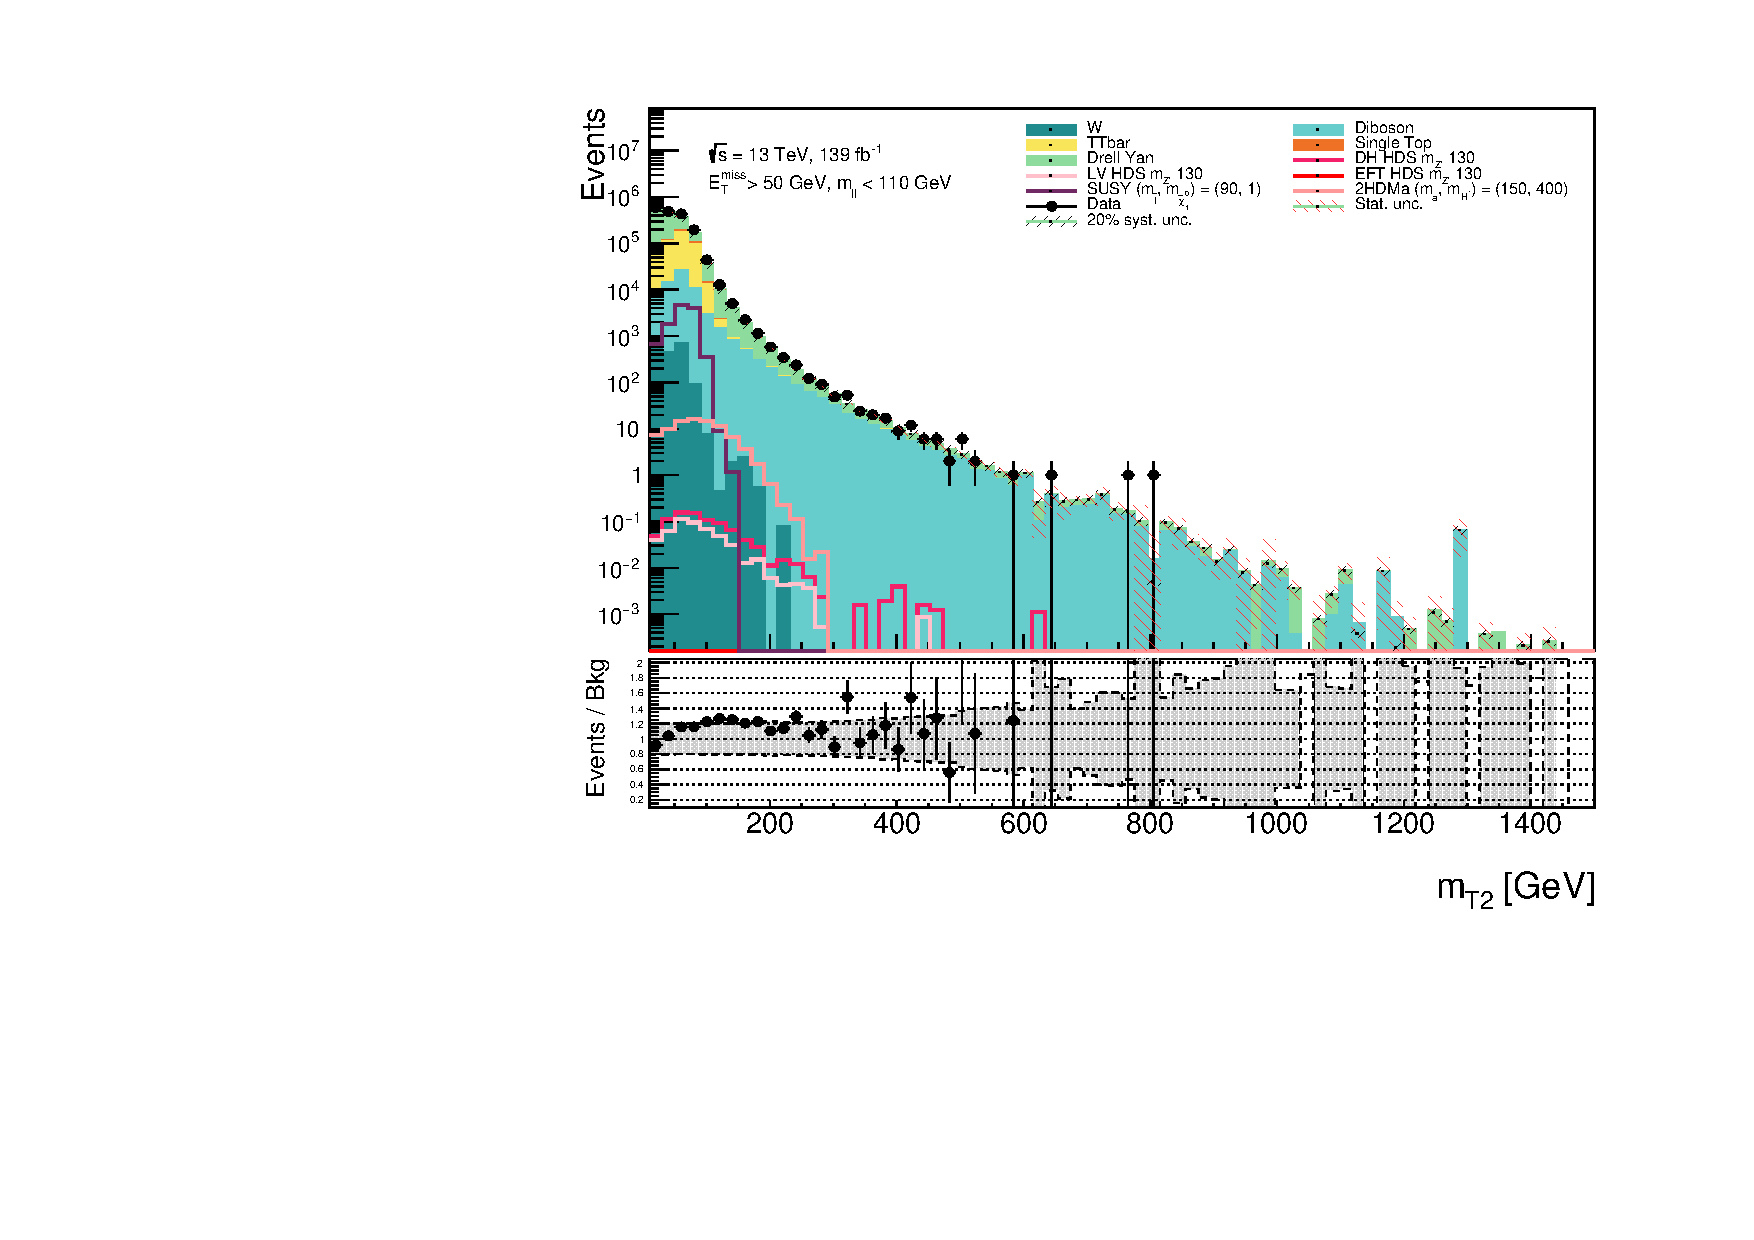
\includegraphics[width=0.8\textwidth]{mt2.pdf}
    \caption{Distribution of $m_{T2}$ in control region.}\label{fig:mt2_dist}
\end{figure}
\\To know the distance between the "lepton-jet" and "MET-jet" we will look at the difference in azimuthal angle between: the lepton pair, $\Delta\Phi(l_1,l_2)$, the dilepton jet and MET jet, $\Delta\Phi(ll,E_T^{miss})$, the leading lepton and MET jet, $\Delta\Phi(l_l,E_T^{miss})$, 
and the lepton closest to the MET jet and the MET jet, $\Delta\Phi(l_c,E_T^{miss})$. In some of the models we are studying it is expected for DM and the leptons pair to be back to back. The distribution of $\Delta\Phi(ll,E_T^{miss})$ can be seen in Figure \ref{fig:dPhiLLMET_dist}.
\begin{figure}[!ht]
    \centering
        \includegraphics[width=0.8\textwidth]{dPhiLLMET.pdf}
    \caption{Distribution of $\Delta\Phi(ll,E_T^{miss})$ in control region.}\label{fig:dPhiLLMET_dist}
\end{figure}

\clearpage\noindent The kinematic variables used are summarized in Table \ref{tab:variables} and the distribution of the remaining kinematical variables are shown in Appendix \ref{apendix:Kin_var_in_CR}.
\begin{table}[!h]
    \centering
    \caption[Kinematic variables used as features]{Table showcasing the kinematic variables that will be used as features on our ML algorithm.\\ * These have poor MC and data agreement. $^\dagger$ These will become a problem when \textit{padding}.}
    \begin{tabular}{l|r}\midrule\midrule
        Kinematic variable                                                              & Feature name          \\\midrule
        $p_T$ of both leptons                                                           & lep1pt \& lep2pt      \\
        $\phi$ of both leptons                                                          & lep1phi \& lep2phi    \\
        $\eta$ of both leptons                                                          & lep1eta \& lep2eta    \\
        Invariant mass of dilepton pair, $m_{ll}$                                       & mll \\
        Missing transverse energy in event, $E_T^{miss}$                                & met \\
        Missing transverse energy significance in event, $E_T^{miss,sig}$               & met\_sig \\
        Transverse mass in in event, $m_T$                                              & mt \\
        Stransverse mass in in event, $m_{T2}$                                          & mt2\\
        Transverse energy of lepton pair, $E_T$                                         & et \\
        $\phi$ between leption pair, $\Delta\Phi(l_1,l_2)$*                             & dPhiLeps \\
        $\phi$ between leption pair and MET jet, $\Delta\Phi(ll,E_T^{miss})$            & dPhiLLMet \\
        $\phi$ between leading lepton and MET jet, $\Delta\Phi(l_l,E_T^{miss})$         & dPhiLeadMet \\
        $\phi$ between closest lepton and MET jet, $\Delta\Phi(l_c,E_T^{miss})$*        & dPhiCloseMet \\
        Hadronic activity, $H_T$                                                        & ht\\
        Ratio between $E_T^{miss}$ and $H_T$                                            & rt\\
        Number of b-jets                                                                & nbjets         \\
        Number of light jets                                                            & nljets         \\
        $p_T$ of three jets with highest $p_T$$^\dagger$                                & jet1pt \& jet2pt \& jet3pt\\
        $\phi$ of three jets with highest $p_T$$^\dagger$                               & jet1phi \& jet2phi \& jet3phi\\
        $\eta$ of three jets with highest $p_T$$^\dagger$                               & jet1eta \& jet2eta \& jet3eta\\
        Invariant mass of two jets with highest $p_T$, $m_{jj}$$^\dagger$               & mjj\\\midrule\midrule
    \end{tabular}
    \label{tab:variables}
\end{table}

\end{document}